\documentclass{article} % For LaTex2e
\usepackage{iclr2022_conference,times}
% Optional math commands from https://github.com/goodfeli/dlbook_notation.
%%%%% NEW MATH DEFINITIONS %%%%%

\usepackage{amsmath,amsfonts,bm}

% Mark sections of captions for referring to divisions of figures
\newcommand{\figleft}{{\em (Left)}}
\newcommand{\figcenter}{{\em (Center)}}
\newcommand{\figright}{{\em (Right)}}
\newcommand{\figtop}{{\em (Top)}}
\newcommand{\figbottom}{{\em (Bottom)}}
\newcommand{\captiona}{{\em (a)}}
\newcommand{\captionb}{{\em (b)}}
\newcommand{\captionc}{{\em (c)}}
\newcommand{\captiond}{{\em (d)}}

% Highlight a newly defined term
\newcommand{\newterm}[1]{{\bf #1}}


% Figure reference, lower-case.
\def\figref#1{figure~\ref{#1}}
% Figure reference, capital. For start of sentence
\def\Figref#1{Figure~\ref{#1}}
\def\twofigref#1#2{figures \ref{#1} and \ref{#2}}
\def\quadfigref#1#2#3#4{figures \ref{#1}, \ref{#2}, \ref{#3} and \ref{#4}}
% Section reference, lower-case.
\def\secref#1{section~\ref{#1}}
% Section reference, capital.
\def\Secref#1{Section~\ref{#1}}
% Reference to two sections.
\def\twosecrefs#1#2{sections \ref{#1} and \ref{#2}}
% Reference to three sections.
\def\secrefs#1#2#3{sections \ref{#1}, \ref{#2} and \ref{#3}}
% Reference to an equation, lower-case.
\def\eqref#1{equation~\ref{#1}}
% Reference to an equation, upper case
\def\Eqref#1{Equation~\ref{#1}}
% A raw reference to an equation---avoid using if possible
\def\plaineqref#1{\ref{#1}}
% Reference to a chapter, lower-case.
\def\chapref#1{chapter~\ref{#1}}
% Reference to an equation, upper case.
\def\Chapref#1{Chapter~\ref{#1}}
% Reference to a range of chapters
\def\rangechapref#1#2{chapters\ref{#1}--\ref{#2}}
% Reference to an algorithm, lower-case.
\def\algref#1{algorithm~\ref{#1}}
% Reference to an algorithm, upper case.
\def\Algref#1{Algorithm~\ref{#1}}
\def\twoalgref#1#2{algorithms \ref{#1} and \ref{#2}}
\def\Twoalgref#1#2{Algorithms \ref{#1} and \ref{#2}}
% Reference to a part, lower case
\def\partref#1{part~\ref{#1}}
% Reference to a part, upper case
\def\Partref#1{Part~\ref{#1}}
\def\twopartref#1#2{parts \ref{#1} and \ref{#2}}

\def\ceil#1{\lceil #1 \rceil}
\def\floor#1{\lfloor #1 \rfloor}
\def\1{\bm{1}}
\newcommand{\train}{\mathcal{D}}
\newcommand{\valid}{\mathcal{D_{\mathrm{valid}}}}
\newcommand{\test}{\mathcal{D_{\mathrm{test}}}}

\def\eps{{\epsilon}}


% Random variables
\def\reta{{\textnormal{$\eta$}}}
\def\ra{{\textnormal{a}}}
\def\rb{{\textnormal{b}}}
\def\rc{{\textnormal{c}}}
\def\rd{{\textnormal{d}}}
\def\re{{\textnormal{e}}}
\def\rf{{\textnormal{f}}}
\def\rg{{\textnormal{g}}}
\def\rh{{\textnormal{h}}}
\def\ri{{\textnormal{i}}}
\def\rj{{\textnormal{j}}}
\def\rk{{\textnormal{k}}}
\def\rl{{\textnormal{l}}}
% rm is already a command, just don't name any random variables m
\def\rn{{\textnormal{n}}}
\def\ro{{\textnormal{o}}}
\def\rp{{\textnormal{p}}}
\def\rq{{\textnormal{q}}}
\def\rr{{\textnormal{r}}}
\def\rs{{\textnormal{s}}}
\def\rt{{\textnormal{t}}}
\def\ru{{\textnormal{u}}}
\def\rv{{\textnormal{v}}}
\def\rw{{\textnormal{w}}}
\def\rx{{\textnormal{x}}}
\def\ry{{\textnormal{y}}}
\def\rz{{\textnormal{z}}}

% Random vectors
\def\rvepsilon{{\mathbf{\epsilon}}}
\def\rvtheta{{\mathbf{\theta}}}
\def\rva{{\mathbf{a}}}
\def\rvb{{\mathbf{b}}}
\def\rvc{{\mathbf{c}}}
\def\rvd{{\mathbf{d}}}
\def\rve{{\mathbf{e}}}
\def\rvf{{\mathbf{f}}}
\def\rvg{{\mathbf{g}}}
\def\rvh{{\mathbf{h}}}
\def\rvu{{\mathbf{i}}}
\def\rvj{{\mathbf{j}}}
\def\rvk{{\mathbf{k}}}
\def\rvl{{\mathbf{l}}}
\def\rvm{{\mathbf{m}}}
\def\rvn{{\mathbf{n}}}
\def\rvo{{\mathbf{o}}}
\def\rvp{{\mathbf{p}}}
\def\rvq{{\mathbf{q}}}
\def\rvr{{\mathbf{r}}}
\def\rvs{{\mathbf{s}}}
\def\rvt{{\mathbf{t}}}
\def\rvu{{\mathbf{u}}}
\def\rvv{{\mathbf{v}}}
\def\rvw{{\mathbf{w}}}
\def\rvx{{\mathbf{x}}}
\def\rvy{{\mathbf{y}}}
\def\rvz{{\mathbf{z}}}

% Elements of random vectors
\def\erva{{\textnormal{a}}}
\def\ervb{{\textnormal{b}}}
\def\ervc{{\textnormal{c}}}
\def\ervd{{\textnormal{d}}}
\def\erve{{\textnormal{e}}}
\def\ervf{{\textnormal{f}}}
\def\ervg{{\textnormal{g}}}
\def\ervh{{\textnormal{h}}}
\def\ervi{{\textnormal{i}}}
\def\ervj{{\textnormal{j}}}
\def\ervk{{\textnormal{k}}}
\def\ervl{{\textnormal{l}}}
\def\ervm{{\textnormal{m}}}
\def\ervn{{\textnormal{n}}}
\def\ervo{{\textnormal{o}}}
\def\ervp{{\textnormal{p}}}
\def\ervq{{\textnormal{q}}}
\def\ervr{{\textnormal{r}}}
\def\ervs{{\textnormal{s}}}
\def\ervt{{\textnormal{t}}}
\def\ervu{{\textnormal{u}}}
\def\ervv{{\textnormal{v}}}
\def\ervw{{\textnormal{w}}}
\def\ervx{{\textnormal{x}}}
\def\ervy{{\textnormal{y}}}
\def\ervz{{\textnormal{z}}}

% Random matrices
\def\rmA{{\mathbf{A}}}
\def\rmB{{\mathbf{B}}}
\def\rmC{{\mathbf{C}}}
\def\rmD{{\mathbf{D}}}
\def\rmE{{\mathbf{E}}}
\def\rmF{{\mathbf{F}}}
\def\rmG{{\mathbf{G}}}
\def\rmH{{\mathbf{H}}}
\def\rmI{{\mathbf{I}}}
\def\rmJ{{\mathbf{J}}}
\def\rmK{{\mathbf{K}}}
\def\rmL{{\mathbf{L}}}
\def\rmM{{\mathbf{M}}}
\def\rmN{{\mathbf{N}}}
\def\rmO{{\mathbf{O}}}
\def\rmP{{\mathbf{P}}}
\def\rmQ{{\mathbf{Q}}}
\def\rmR{{\mathbf{R}}}
\def\rmS{{\mathbf{S}}}
\def\rmT{{\mathbf{T}}}
\def\rmU{{\mathbf{U}}}
\def\rmV{{\mathbf{V}}}
\def\rmW{{\mathbf{W}}}
\def\rmX{{\mathbf{X}}}
\def\rmY{{\mathbf{Y}}}
\def\rmZ{{\mathbf{Z}}}

% Elements of random matrices
\def\ermA{{\textnormal{A}}}
\def\ermB{{\textnormal{B}}}
\def\ermC{{\textnormal{C}}}
\def\ermD{{\textnormal{D}}}
\def\ermE{{\textnormal{E}}}
\def\ermF{{\textnormal{F}}}
\def\ermG{{\textnormal{G}}}
\def\ermH{{\textnormal{H}}}
\def\ermI{{\textnormal{I}}}
\def\ermJ{{\textnormal{J}}}
\def\ermK{{\textnormal{K}}}
\def\ermL{{\textnormal{L}}}
\def\ermM{{\textnormal{M}}}
\def\ermN{{\textnormal{N}}}
\def\ermO{{\textnormal{O}}}
\def\ermP{{\textnormal{P}}}
\def\ermQ{{\textnormal{Q}}}
\def\ermR{{\textnormal{R}}}
\def\ermS{{\textnormal{S}}}
\def\ermT{{\textnormal{T}}}
\def\ermU{{\textnormal{U}}}
\def\ermV{{\textnormal{V}}}
\def\ermW{{\textnormal{W}}}
\def\ermX{{\textnormal{X}}}
\def\ermY{{\textnormal{Y}}}
\def\ermZ{{\textnormal{Z}}}

% Vectors
\def\vzero{{\bm{0}}}
\def\vone{{\bm{1}}}
\def\vmu{{\bm{\mu}}}
\def\vtheta{{\bm{\theta}}}
\def\va{{\bm{a}}}
\def\vb{{\bm{b}}}
\def\vc{{\bm{c}}}
\def\vd{{\bm{d}}}
\def\ve{{\bm{e}}}
\def\vf{{\bm{f}}}
\def\vg{{\bm{g}}}
\def\vh{{\bm{h}}}
\def\vi{{\bm{i}}}
\def\vj{{\bm{j}}}
\def\vk{{\bm{k}}}
\def\vl{{\bm{l}}}
\def\vm{{\bm{m}}}
\def\vn{{\bm{n}}}
\def\vo{{\bm{o}}}
\def\vp{{\bm{p}}}
\def\vq{{\bm{q}}}
\def\vr{{\bm{r}}}
\def\vs{{\bm{s}}}
\def\vt{{\bm{t}}}
\def\vu{{\bm{u}}}
\def\vv{{\bm{v}}}
\def\vw{{\bm{w}}}
\def\vx{{\bm{x}}}
\def\vy{{\bm{y}}}
\def\vz{{\bm{z}}}

% Elements of vectors
\def\evalpha{{\alpha}}
\def\evbeta{{\beta}}
\def\evepsilon{{\epsilon}}
\def\evlambda{{\lambda}}
\def\evomega{{\omega}}
\def\evmu{{\mu}}
\def\evpsi{{\psi}}
\def\evsigma{{\sigma}}
\def\evtheta{{\theta}}
\def\eva{{a}}
\def\evb{{b}}
\def\evc{{c}}
\def\evd{{d}}
\def\eve{{e}}
\def\evf{{f}}
\def\evg{{g}}
\def\evh{{h}}
\def\evi{{i}}
\def\evj{{j}}
\def\evk{{k}}
\def\evl{{l}}
\def\evm{{m}}
\def\evn{{n}}
\def\evo{{o}}
\def\evp{{p}}
\def\evq{{q}}
\def\evr{{r}}
\def\evs{{s}}
\def\evt{{t}}
\def\evu{{u}}
\def\evv{{v}}
\def\evw{{w}}
\def\evx{{x}}
\def\evy{{y}}
\def\evz{{z}}

% Matrix
\def\mA{{\bm{A}}}
\def\mB{{\bm{B}}}
\def\mC{{\bm{C}}}
\def\mD{{\bm{D}}}
\def\mE{{\bm{E}}}
\def\mF{{\bm{F}}}
\def\mG{{\bm{G}}}
\def\mH{{\bm{H}}}
\def\mI{{\bm{I}}}
\def\mJ{{\bm{J}}}
\def\mK{{\bm{K}}}
\def\mL{{\bm{L}}}
\def\mM{{\bm{M}}}
\def\mN{{\bm{N}}}
\def\mO{{\bm{O}}}
\def\mP{{\bm{P}}}
\def\mQ{{\bm{Q}}}
\def\mR{{\bm{R}}}
\def\mS{{\bm{S}}}
\def\mT{{\bm{T}}}
\def\mU{{\bm{U}}}
\def\mV{{\bm{V}}}
\def\mW{{\bm{W}}}
\def\mX{{\bm{X}}}
\def\mY{{\bm{Y}}}
\def\mZ{{\bm{Z}}}
\def\mBeta{{\bm{\beta}}}
\def\mPhi{{\bm{\Phi}}}
\def\mLambda{{\bm{\Lambda}}}
\def\mSigma{{\bm{\Sigma}}}

% Tensor
\DeclareMathAlphabet{\mathsfit}{\encodingdefault}{\sfdefault}{m}{sl}
\SetMathAlphabet{\mathsfit}{bold}{\encodingdefault}{\sfdefault}{bx}{n}
\newcommand{\tens}[1]{\bm{\mathsfit{#1}}}
\def\tA{{\tens{A}}}
\def\tB{{\tens{B}}}
\def\tC{{\tens{C}}}
\def\tD{{\tens{D}}}
\def\tE{{\tens{E}}}
\def\tF{{\tens{F}}}
\def\tG{{\tens{G}}}
\def\tH{{\tens{H}}}
\def\tI{{\tens{I}}}
\def\tJ{{\tens{J}}}
\def\tK{{\tens{K}}}
\def\tL{{\tens{L}}}
\def\tM{{\tens{M}}}
\def\tN{{\tens{N}}}
\def\tO{{\tens{O}}}
\def\tP{{\tens{P}}}
\def\tQ{{\tens{Q}}}
\def\tR{{\tens{R}}}
\def\tS{{\tens{S}}}
\def\tT{{\tens{T}}}
\def\tU{{\tens{U}}}
\def\tV{{\tens{V}}}
\def\tW{{\tens{W}}}
\def\tX{{\tens{X}}}
\def\tY{{\tens{Y}}}
\def\tZ{{\tens{Z}}}


% Graph
\def\gA{{\mathcal{A}}}
\def\gB{{\mathcal{B}}}
\def\gC{{\mathcal{C}}}
\def\gD{{\mathcal{D}}}
\def\gE{{\mathcal{E}}}
\def\gF{{\mathcal{F}}}
\def\gG{{\mathcal{G}}}
\def\gH{{\mathcal{H}}}
\def\gI{{\mathcal{I}}}
\def\gJ{{\mathcal{J}}}
\def\gK{{\mathcal{K}}}
\def\gL{{\mathcal{L}}}
\def\gM{{\mathcal{M}}}
\def\gN{{\mathcal{N}}}
\def\gO{{\mathcal{O}}}
\def\gP{{\mathcal{P}}}
\def\gQ{{\mathcal{Q}}}
\def\gR{{\mathcal{R}}}
\def\gS{{\mathcal{S}}}
\def\gT{{\mathcal{T}}}
\def\gU{{\mathcal{U}}}
\def\gV{{\mathcal{V}}}
\def\gW{{\mathcal{W}}}
\def\gX{{\mathcal{X}}}
\def\gY{{\mathcal{Y}}}
\def\gZ{{\mathcal{Z}}}

% Sets
\def\sA{{\mathbb{A}}}
\def\sB{{\mathbb{B}}}
\def\sC{{\mathbb{C}}}
\def\sD{{\mathbb{D}}}
% Don't use a set called E, because this would be the same as our symbol
% for expectation.
\def\sF{{\mathbb{F}}}
\def\sG{{\mathbb{G}}}
\def\sH{{\mathbb{H}}}
\def\sI{{\mathbb{I}}}
\def\sJ{{\mathbb{J}}}
\def\sK{{\mathbb{K}}}
\def\sL{{\mathbb{L}}}
\def\sM{{\mathbb{M}}}
\def\sN{{\mathbb{N}}}
\def\sO{{\mathbb{O}}}
\def\sP{{\mathbb{P}}}
\def\sQ{{\mathbb{Q}}}
\def\sR{{\mathbb{R}}}
\def\sS{{\mathbb{S}}}
\def\sT{{\mathbb{T}}}
\def\sU{{\mathbb{U}}}
\def\sV{{\mathbb{V}}}
\def\sW{{\mathbb{W}}}
\def\sX{{\mathbb{X}}}
\def\sY{{\mathbb{Y}}}
\def\sZ{{\mathbb{Z}}}

% Entries of a matrix
\def\emLambda{{\Lambda}}
\def\emA{{A}}
\def\emB{{B}}
\def\emC{{C}}
\def\emD{{D}}
\def\emE{{E}}
\def\emF{{F}}
\def\emG{{G}}
\def\emH{{H}}
\def\emI{{I}}
\def\emJ{{J}}
\def\emK{{K}}
\def\emL{{L}}
\def\emM{{M}}
\def\emN{{N}}
\def\emO{{O}}
\def\emP{{P}}
\def\emQ{{Q}}
\def\emR{{R}}
\def\emS{{S}}
\def\emT{{T}}
\def\emU{{U}}
\def\emV{{V}}
\def\emW{{W}}
\def\emX{{X}}
\def\emY{{Y}}
\def\emZ{{Z}}
\def\emSigma{{\Sigma}}

% entries of a tensor
% Same font as tensor, without \bm wrapper
\newcommand{\etens}[1]{\mathsfit{#1}}
\def\etLambda{{\etens{\Lambda}}}
\def\etA{{\etens{A}}}
\def\etB{{\etens{B}}}
\def\etC{{\etens{C}}}
\def\etD{{\etens{D}}}
\def\etE{{\etens{E}}}
\def\etF{{\etens{F}}}
\def\etG{{\etens{G}}}
\def\etH{{\etens{H}}}
\def\etI{{\etens{I}}}
\def\etJ{{\etens{J}}}
\def\etK{{\etens{K}}}
\def\etL{{\etens{L}}}
\def\etM{{\etens{M}}}
\def\etN{{\etens{N}}}
\def\etO{{\etens{O}}}
\def\etP{{\etens{P}}}
\def\etQ{{\etens{Q}}}
\def\etR{{\etens{R}}}
\def\etS{{\etens{S}}}
\def\etT{{\etens{T}}}
\def\etU{{\etens{U}}}
\def\etV{{\etens{V}}}
\def\etW{{\etens{W}}}
\def\etX{{\etens{X}}}
\def\etY{{\etens{Y}}}
\def\etZ{{\etens{Z}}}

% The true underlying data generating distribution
\newcommand{\pdata}{p_{\rm{data}}}
% The empirical distribution defined by the training set
\newcommand{\ptrain}{\hat{p}_{\rm{data}}}
\newcommand{\Ptrain}{\hat{P}_{\rm{data}}}
% The model distribution
\newcommand{\pmodel}{p_{\rm{model}}}
\newcommand{\Pmodel}{P_{\rm{model}}}
\newcommand{\ptildemodel}{\tilde{p}_{\rm{model}}}
% Stochastic autoencoder distributions
\newcommand{\pencode}{p_{\rm{encoder}}}
\newcommand{\pdecode}{p_{\rm{decoder}}}
\newcommand{\precons}{p_{\rm{reconstruct}}}

\newcommand{\laplace}{\mathrm{Laplace}} % Laplace distribution

\newcommand{\E}{\mathbb{E}}
\newcommand{\Ls}{\mathcal{L}}
\newcommand{\R}{\mathbb{R}}
\newcommand{\emp}{\tilde{p}}
\newcommand{\lr}{\alpha}
\newcommand{\reg}{\lambda}
\newcommand{\rect}{\mathrm{rectifier}}
\newcommand{\softmax}{\mathrm{softmax}}
\newcommand{\sigmoid}{\sigma}
\newcommand{\softplus}{\zeta}
\newcommand{\KL}{D_{\mathrm{KL}}}
\newcommand{\Var}{\mathrm{Var}}
\newcommand{\standarderror}{\mathrm{SE}}
\newcommand{\Cov}{\mathrm{Cov}}
% Wolfram Mathworld says $L^2$ is for function spaces and $\ell^2$ is for vectors
% But then they seem to use $L^2$ for vectors throughout the site, and so does
% wikipedia.
\newcommand{\normlzero}{L^0}
\newcommand{\normlone}{L^1}
\newcommand{\normltwo}{L^2}
\newcommand{\normlp}{L^p}
\newcommand{\normmax}{L^\infty}

\newcommand{\parents}{Pa} % See usage in notation.tex. Chosen to match Daphne's book.

\DeclareMathOperator*{\argmax}{arg\,max}
\DeclareMathOperator*{\argmin}{arg\,min}

\DeclareMathOperator{\sign}{sign}
\DeclareMathOperator{\Tr}{Tr}
\let\ab\allowbreak


%######## APS360: Uncomment your submission name
%\newcommand{\apsname}{Project Proposal}
%\newcommand{\apsname}{Progress Report}
\newcommand{\apsname}{Final Report}

%######## APS360: Put your Group Number here
\newcommand{\gpnumber}{40}

\usepackage{hyperref}
\usepackage{xcolor}
\usepackage[normalem]{ulem}
\usepackage{url}
\usepackage{graphicx}
\usepackage{placeins}
\usepackage{float}
\usepackage{tikz}

%######## APS360: Put your project Title here
\title{Image Colourization via Convolutional \\
Neural Networks and Deep Learning}

%######## APS360: Put your names, student IDs and Emails here
\author{Youssef Fikry  \\
Student\# 1006682626\\
\texttt{youssef.fikry@mail.utoronto.ca} \\
\And Harkirpa Kaur  \\
Student\# 1011242479 \\
\texttt{harkirpa.kaur@mail.utoronto.ca} \\
\AND
Peter Leong \\
Student\# 1010892955 \\
\texttt{peter.leong@mail.utoronto.ca} \\
\And
Thulasi Thavarajah \\
Student\# 1011358424 \\
\texttt{t.thavarajah@mail.utoronto.ca} \\
\AND
}

% The \author macro works with any number of authors. There are two commands
% used to separate the names and addresses of multiple authors: \And and \AND.
%
% Using \And between authors leaves it to \LaTex{} to determine where to break
% the lines. Using \AND forces a linebreak at that point. So, if \LaTex{}
% puts 3 of 4 authors names on the first line, and the last on the second
% line, try using \AND instead of \And before the third author name.

\newcommand{\fix}{\marginpar{FIx}}
\newcommand{\new}{\marginpar{NEW}}

\iclrfinalcopy 
%######## APS360: Document starts here
\begin{document}

\maketitle

\begin{abstract}
This project addresses the challenge of automated colourization for 256$\times$256 grayscale images using a dataset of 12,600 image pairs, balanced across human subjects, 
animals, and natural scenery. We frame colourization as a supervised learning problem in the CIELAB colour space, where a model predicts chrominance channels ($a^*$, $b^*$) 
from the luminance channel ($L^*$). A shallow convolutional neural network (CNN) provides the baseline performance, while our primary solution employs a deeper convolutional 
encoder-decoder architecture. This design captures high-level semantic features and spatial context, addressing limitations of shallow networks in perceptual realism.
%######## APS360: Do not change the next line. This shows your Main body page count.
----Total Pages: \pageref{last_page}
\end{abstract}

\section{Introduction}

While colour photography processes first emerged in the 1890s, colour photography did not become widely accessible until the 1970s \citep{scienceandmediamuseum2020}. 
Consequently, most historical photographs remain in black and white, lacking the visual richness that modern viewers are accustomed to. Moreover, individuals who undergo cataract 
removal as part of vision restoration procedures often struggle to interpret grayscale images, rendering many historical photographs inaccessible to them \citet{vogelsang2024impact}. 
This project aims to leverage deep learning to automatically colourize black and white images, with the goal of restoring visual information and improving accessibility for all audiences. 
Traditional, non-deep learning colourization methods tend to produce desaturated results and require extensive human input, limiting their scalability \citep{cheng2016deepcolorization}. 
In contrast, deep neural networks such as convolutional neural networks (CNNs) can effectively learn spatial and semantic features, enabling realistic colourization without user 
intervention \citep{zhang2016colorful}. This makes deep learning a promising and scalable solution for image colourization.

\section{Background \& Related Work}

The challenge of image colourization has been addressed through a range of methods, particularly within deep learning. Even among deep learning-based solutions, researchers 
have proposed a variety of architectures, which can be broadly categorized into five groups: simple colourization neural networks, user-guided colourization networks, diverse 
colourization networks, multi-path networks, and exemplar-based approaches \citep{zeger2021grayscale}.

Simple colourization neural networks use feedforward convolutional neural networks (CNNs) to directly map grayscale inputs to colour outputs. One of the most influential examples 
is the work by \citet{zhang2016colorful}, who proposed a fully convolutional network that predicts the \textit{a} and \textit{b} channels in the CIELAB colour space. Their 
architecture comprises several convolutional layers, each followed by ReLU activations and batch normalization, and is trained as a classification task over quantized ab values, 
producing more vivid outputs than regression-based methods.

User-guided colourization networks incorporate human input to guide the colourization process. \citet{zhang2017real} extended their earlier work by accepting user-provided colour 
“scribbles” as input alongside the grayscale image. The network learns to propagate these hints across the image while minimizing differences from the target colour, allowing 
interactive and controllable colourization.

Diverse colourization networks aim to generate multiple plausible colourizations for a single grayscale input. For instance, \citet{Vitoria2020ChromaGAN} used a generative adversarial 
network (GAN) to produce diverse outputs by learning a conditional distribution over colourizations. This approach addresses the inherent ambiguity in mapping grayscale to colour.

Multi-path colourization networks extract features at multiple spatial resolutions to improve accuracy and context-awareness. \citet{Iizuka2016Colourization} proposed a model with both 
global and local feature pathways, enabling the network to learn both scene-level semantics and fine-grained textures. This structure helps ensure coherent colourization across different 
image regions.

Exemplar-based colourization networks transfer colour information from reference images to the target. In \citet{su2020instanceawareimagecolorization}, instance segmentation is used 
to match regions between the target and exemplars, and two separate colourization networks process this information before merging their outputs. This instance-level guidance simplifies 
the task compared to end-to-end full-image colourization and enhances accuracy in semantically similar scenes.

\section{Data Processing}

 The project's image dataset was compiled using publicly available datasets on Kaggle.com, an online platform that provides access to real-world datasets and a community for data 
 scientists \citep[]{kaggle}. To train a model that can generalize to a broad range of images, the final dataset for this project includes three categories: human, animal, and scenic. 
 All selected datasets are licensed for public domain use. 

\subsection{Repurposing Online Datasets}

The human image dataset, originally intended for human detection, contains a diverse range of 17,300 images of people in different environments \citep[]{kaggle_human}. Furthermore, 
the animal image dataset, initially developed for image classification contains 5,400 images of 90 different animals \citep[]{kaggle_animal}. For this project's purpose, this dataset 
is ideal as it encompasses a diverse set of images with an equal distribution of each animal. Additionally, the scenic image dataset from \citet{kaggle_scene} contains 4,319 images of 
a variety of landscapes spanning a large breadth of colour palettes, potentially influencing the robustness of the final model.

\subsection{Cleaning Up The Datasets}
The team extracted all the images from each dataset and relocated them into folders corresponding to their category (human/animal/scenic). Due to the disparity in the size of the 
three datasets, each dataset was reduced to exactly 4200 images using Python's \verb|random.sample| function with the seed set to 42. The images were then renamed in accordance to 
their respective categories (ex. human\_0001.jpg). 

\begin{figure}[htbp]            % h=here, t=top, b=bottom, p=page float
  \centering
  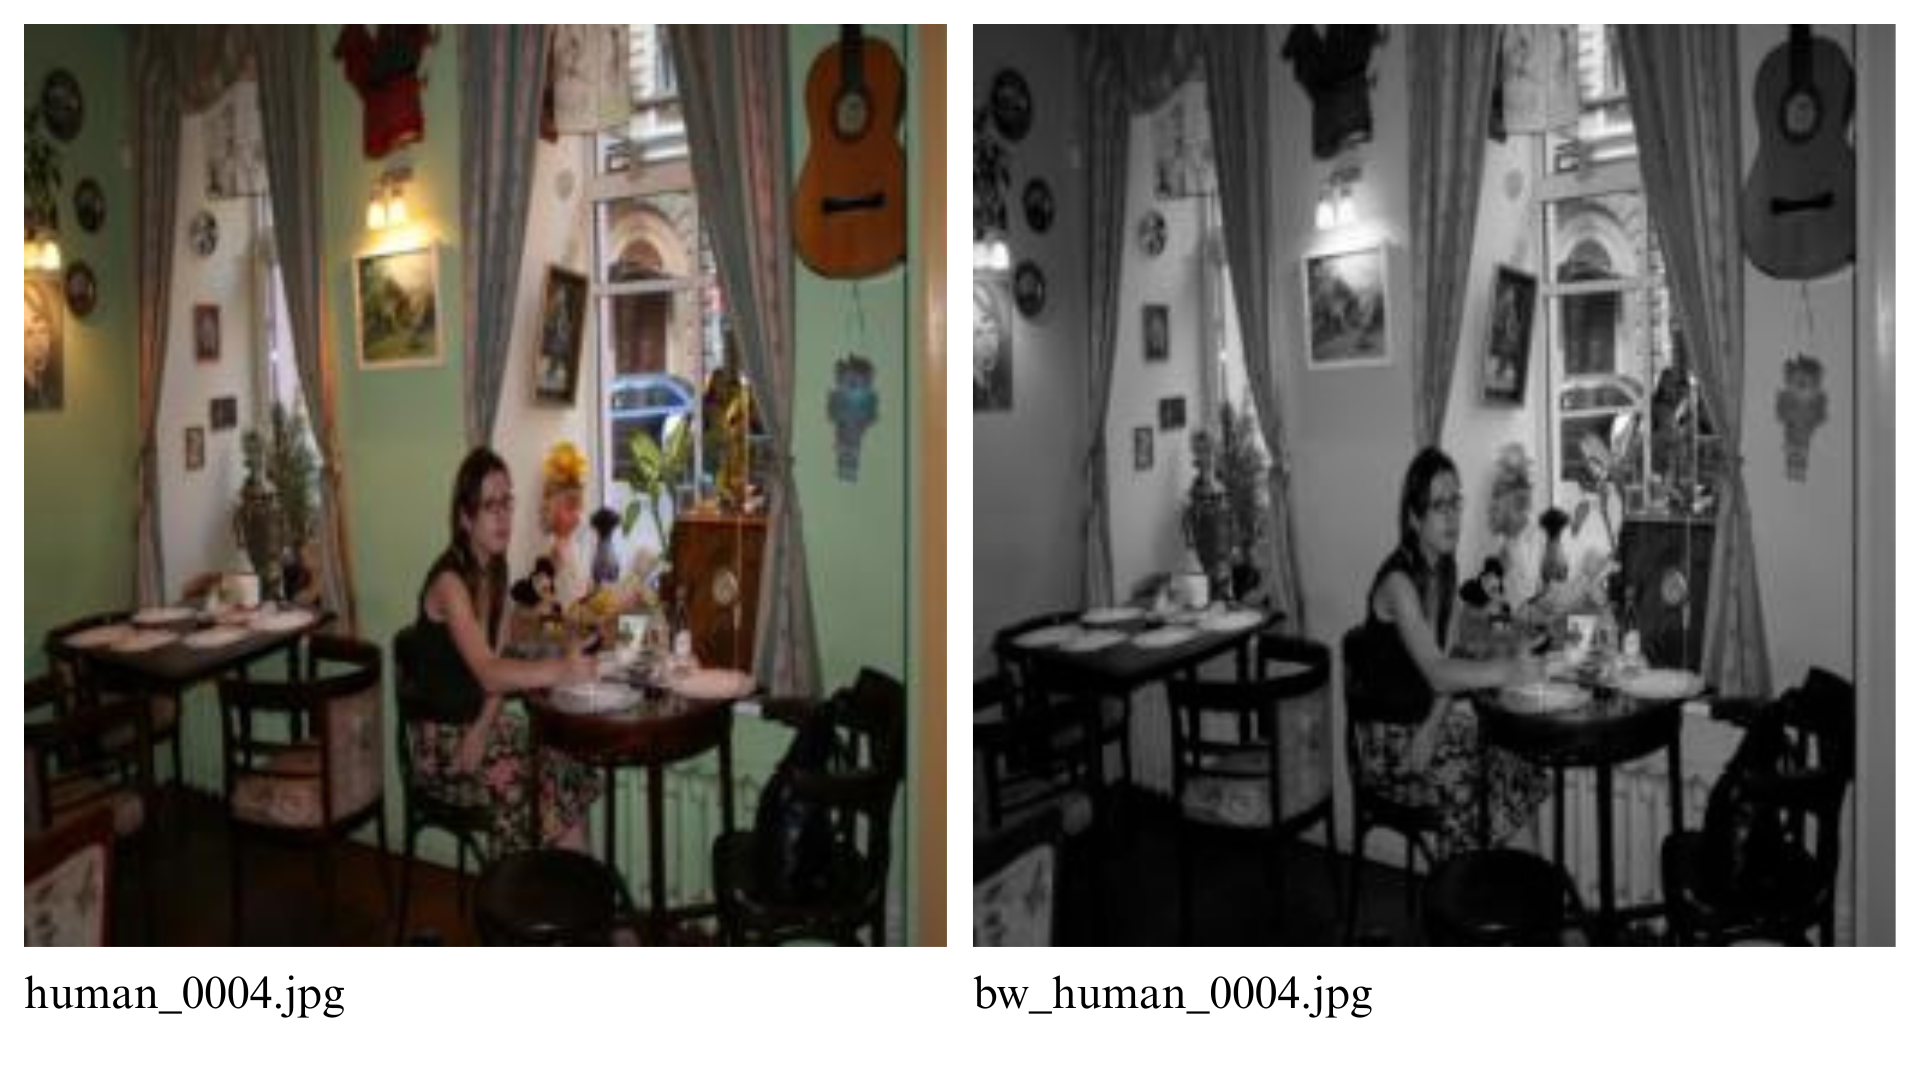
\includegraphics[width=1\linewidth]{Figs/Data Example.png}
  \caption{Sample Data Pair from Training Set}
  \label{fig:data_example}
\end{figure}

\subsection{Formatting the Data}

This project requires a unique dataset with black-and-white images paired with their coloured counterparts as the ground truths. To format the cleaned up data and create this dataset, 
PyTorch's \verb|torchvision.transforms| library was utiltized. The team first converted the original images into 256 x 256 pixel ground truth images using the \verb|Resize| transform 
and sorted them according to their category. Subsequently, the \verb|Grayscale| transform (output channel = 1) converted the 256$\times$256 pixel colour images into grayscale for input 
to the model.

\subsection{Splitting Dataset Into Training, Validation and Test Sets}

The datasets were split into training, validation, and test sets in a 70:15:15 ratio. For each category (human, animal, scene), the first 2940 images formed the training set, with the 
restsplit evenly between validation and testing.

\subsection{The Final Dataset}

The final dataset contains 12{,}600 colour-grayscale image pairs, evenly divided into three categories (human, animal, scenic) with 4{,}200 pairs each. Category balance was maintained 
across the training, validation, and test sets, illustrated in Figure~\ref{fig:data_split}. 

\begin{figure}[h]
\centering
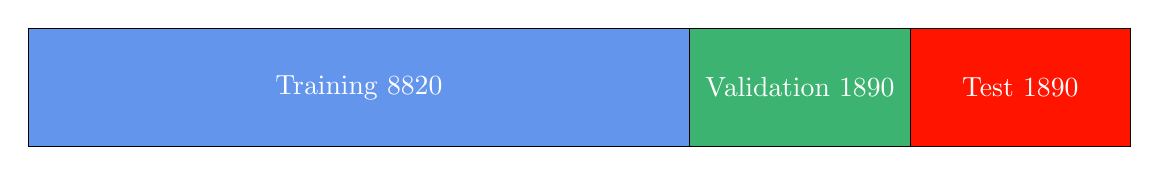
\begin{tikzpicture}
% Define colours
\definecolor{traincol}{RGB}{100,149,237}   % Cornflower blue
\definecolor{valcol}{RGB}{60,179,113}     % Medium sea green
\definecolor{testcol}{RGB}{255,20,0}      % Red

% Total width and height of bar
\newlength{\totalwidth}
\setlength{\totalwidth}{14cm}
\newlength{\barheight}
\setlength{\barheight}{1.5cm}

% Widths proportional to 70:15:15
\newlength{\trainwidth}
\setlength{\trainwidth}{0.6\totalwidth}
\newlength{\valwidth}
\setlength{\valwidth}{0.2\totalwidth}
\newlength{\testwidth}
\setlength{\testwidth}{0.2\totalwidth}

% Draw stacked bar
\draw[fill=traincol] (0,0) rectangle (\trainwidth,\barheight) node[midway,white]{Training 8820};
\draw[fill=valcol] (\trainwidth,0) rectangle (\trainwidth+\valwidth,\barheight) node[midway,white]{Validation 1890};
\draw[fill=testcol] (\trainwidth+\valwidth,0) rectangle (\totalwidth,\barheight) node[midway,white]{Test 1890};

% Outline
\draw (0,0) rectangle (\totalwidth,\barheight);
\end{tikzpicture}
\caption{Distribution of 12{,}600 image pairs across training, validation, and test sets.}
\label{fig:data_split}
\end{figure}

\section{Architecture}

Our primary colourization model is a convolutional encoder-decoder network, a common architecture for image-to-image translation \citep{leatvanich2025image}. Operating in the CIELAB colour 
space, the model takes the L channel (perceptual lightness) as input and predicts the a and b chrominance channels. To ensure input-target consistency, the L channel is derived directly 
from the same RGB image used to generate the ground truth a,b channels. The predicted chrominance is then combined with the L channel and converted back to RGB for visualization. Using 
LAB space decouples intensity from colour, aligns with human perception, and typically produces more realistic results than RGB-based models \citep{leatvanich2025image}.

The architecture is a simplified U-Net. The encoder uses convolutional layers with ReLU activations and batch normalization to progressively downsample the input while extracting high-level 
features. It begins with a 3$\times$3 convolution producing 64 feature maps, followed by layers with increasing filter counts (e.g., 128) that halve spatial resolution. A bottleneck with 256 
filters captures abstract representations. The decoder upsamples back to the original resolution using transposed convolutions to predict the a,b channels, with skip connections preserving 
edges and textures \citep{leatvanich2025image}.

We initialize the encoder with ResNet-18 weights pretrained on ImageNet, leveraging semantic features learned from large-scale datasets to better infer plausible colours for common objects 
\citep{olah2022lettherebecolor}. The decoder and output layers are trained from scratch.

Rather than classifying discrete colour bins \citep{olah2022lettherebecolor}, we use a regression-based approach that directly predicts continuous a,b values. The output head is linear without 
\verb|tanh| activation, avoiding chroma saturation and preserving the full colour range.

To promote vibrant, diverse colourization and reduce bias toward brownish tones, we use a weighted colour loss informed by a dataset-wide chrominance prior. A robust (Huber) pixel loss further 
improves performance by handling uncertainty and avoiding bias toward low-chroma predictions. All augmentations are applied consistently to input and target images, with vertical flips excluded 
to preserve semantic orientation. To shorten training, prior computations are cached and updated once per epoch, reducing runtime from six hours to one.

\section{Illustration}

The top row shows the encoder, consisting of blocks with two convolutional layers followed by max pooling, progressively downsampling the grayscale L channel from 256$\times$256 to 
32$\times$32 while increasing feature depth from 64 to 512. The bottom row shows the decoder, which uses upsampling blocks to restore full resolution and predict the two chrominance channels 
(a and b). Coloured arrows mark four skip connections that transfer fine-grained features from encoder layers to corresponding decoder stages (see Figure~\ref{fig:architecture}).

\begin{figure}[H]
  \centering
  \vspace{-1em} % reduce space before figure
  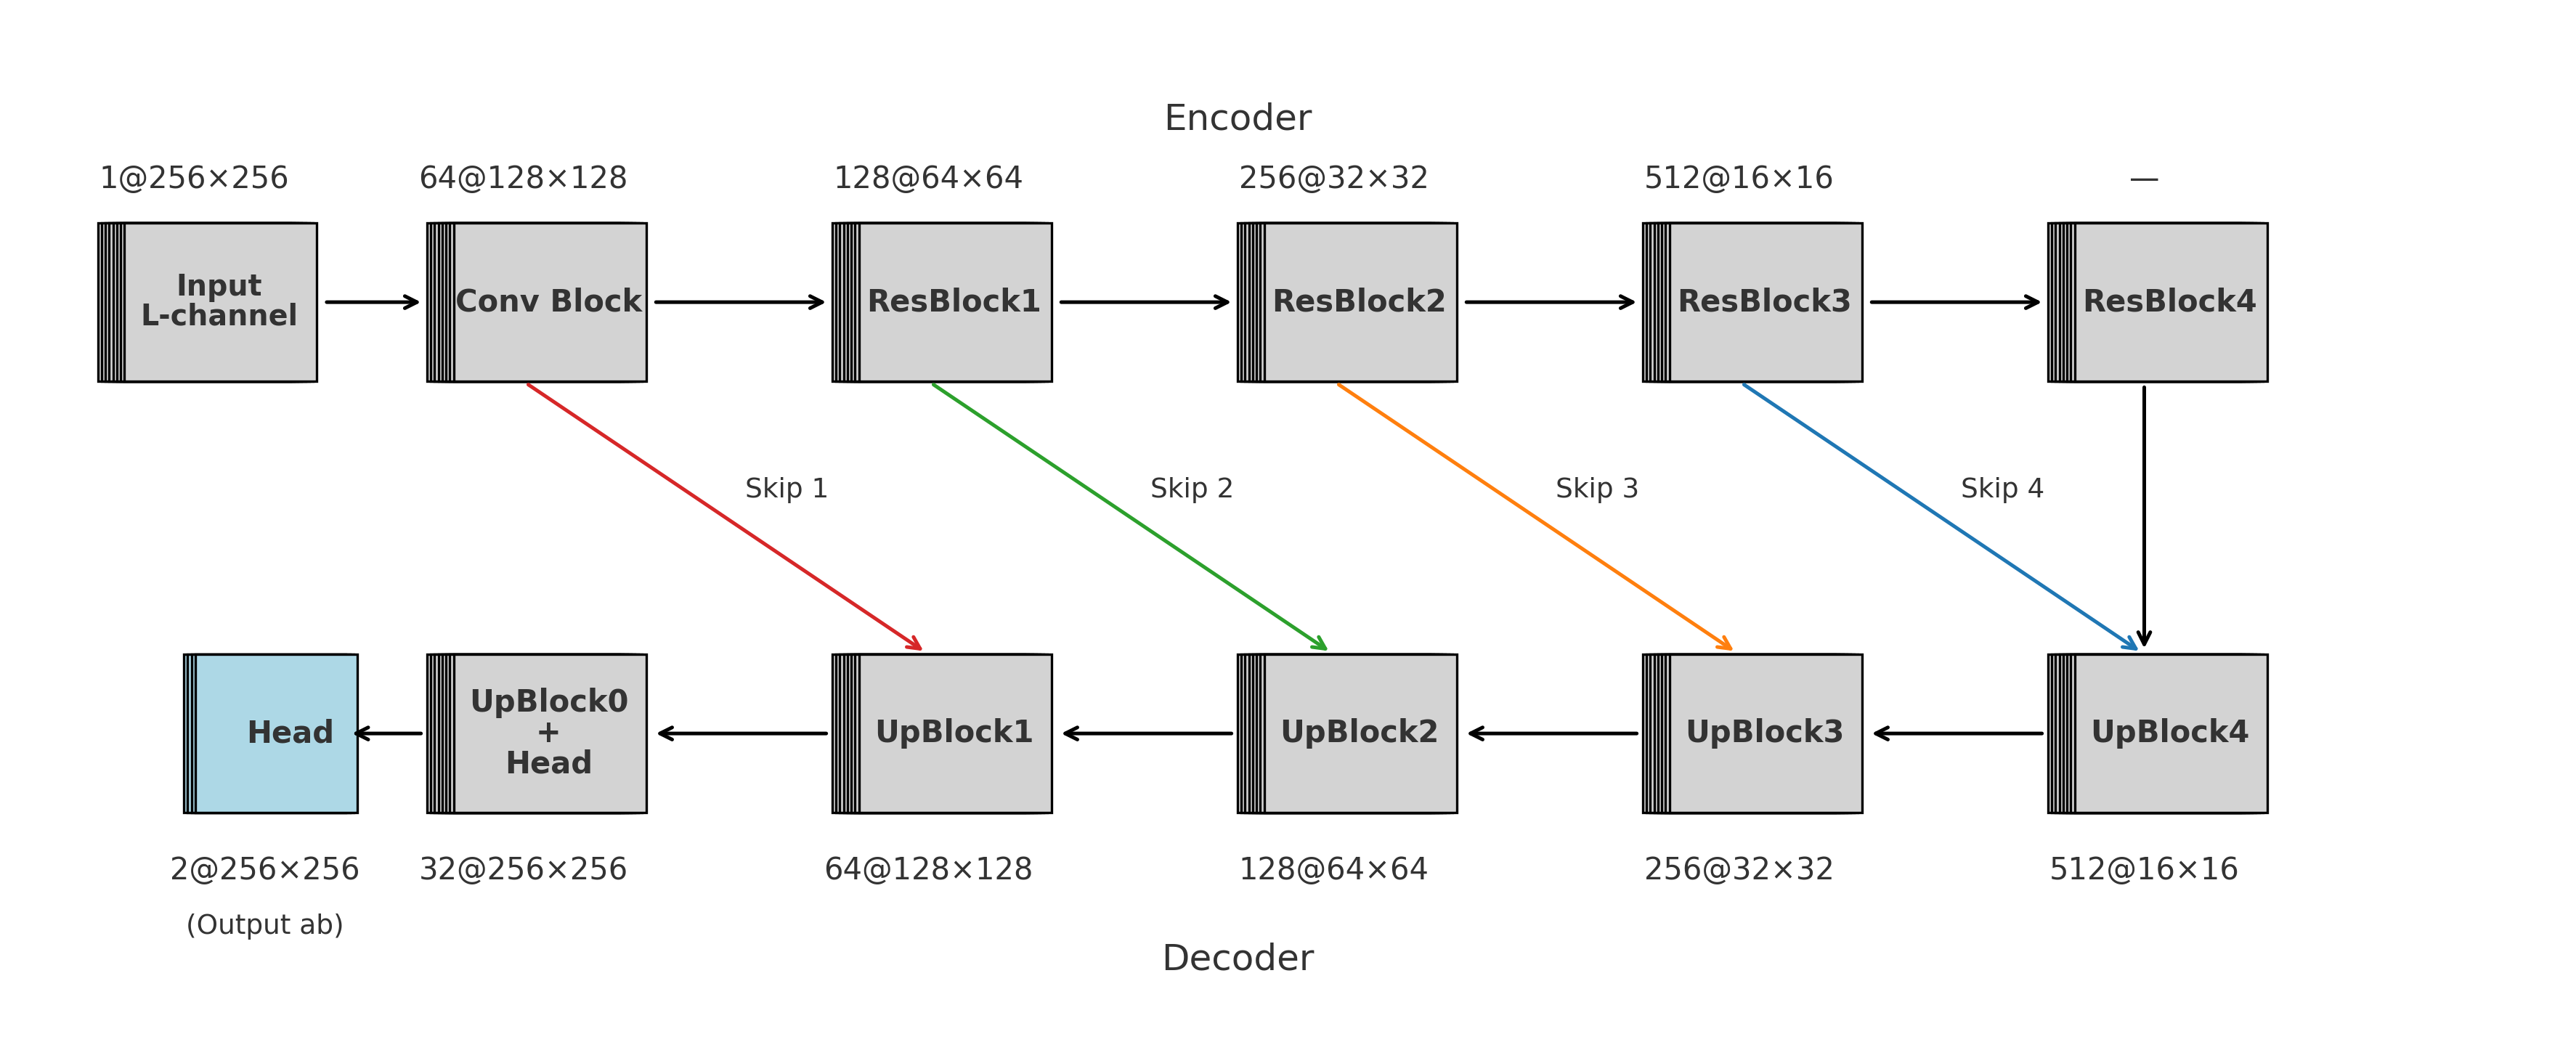
\includegraphics[width=1.1\linewidth]{Figs/architecture-diagram.png}
  \vspace{-0.5em} % reduce space before caption
  \caption{Encoder–decoder colourization network with skip connections from encoder to decoder stages, 
  enabling transfer of fine-grained features during upsampling.}
  \label{fig:architecture}
\end{figure}

\section{Baseline Model}
\label{baseline}

Our baseline was a shallow encoder-decoder convolutional network, designed to be lightweight and fast to train. The model took the L channel of a grayscale image as input and predicted 
the a and b chrominance channels. The encoder had two convolutional layers: the first mapped the input to 64 channels using a 3$\times$3 kernel with padding 1 and ReLU activation, and the 
second expanded to 128 channels with the same kernel and activation. A max-pooling layer with 2$\times$2 kernel and stride 2 halved the spatial resolution, followed by a bottleneck layer 
with 256 filters and ReLU activation to process the compressed features \citep{leatvanich2025image}.

The decoder upsampled the features using a transposed convolution that reduced channels from 256 to 128 while restoring resolution, followed by ReLU. A final convolution projected to 2 
output channels for the a and b values, with Tanh activation to constrain outputs to the normalized LAB range [-1,1] \citep{rosebrock2019bwcolorization}.

No architectural or hyperparameter changes were made to this baseline. It lacked skip connections, pretrained components, or deep feature extraction, and often produced desaturated results. 
Nevertheless, it provided a clear, reproducible benchmark to evaluate improvements from our full model.

\section{Quantitative Results}
\label{quant_results}

We used a combination of smooth loss and colourfullness metric to calculate the loss values for our model. The colourfullness metric encouraged the model to use more saturated colours
instead of resorting to brown hues, which is an issue we previously encountered. 

Validation and training loss was documented after every epoch and the results were graphed, as shown in Figure~\ref{fig:loss_curve}. We observed some overfitting, as the final 
training loss was 0.004423, and the final validation loss was 0.007595.

\begin{figure}[htbp]            % h=here, t=top, b=bottom, p=page float
  \centering
  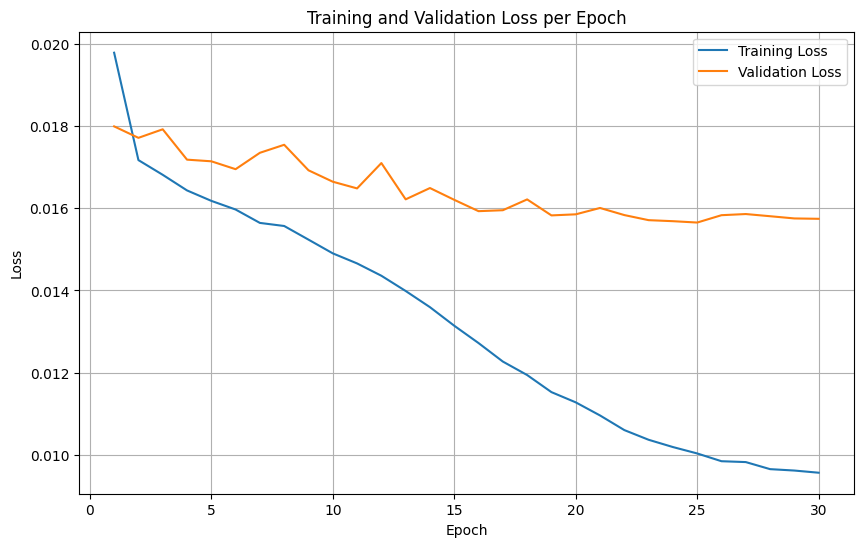
\includegraphics[width=0.9\linewidth]{Figs/loss_curve.png}
  \caption{Learning curve showing training and validation loss over 30 epochs. Validation loss converges after about 15 epochs while training loss continues to decrease, indicating slight overfitting.}
  \label{fig:loss_curve}
\end{figure}

\section{Qualitative Results}
\label{qual_results}

Our primary model consistently outperformed the baseline, particularly on landscape scenes where the network recovered vibrant skies, foliage, and water with relatively realistic hues, 
while the baseline produced dull or grayish outputs lacking semantic colour cues. In many cases, the primary model introduced plausible blue and green tones, suggesting it successfully 
learned common associations between luminance and scene content (see Figure~\ref{fig:landscape_comparison}).

\begin{figure}[H]
  \centering
  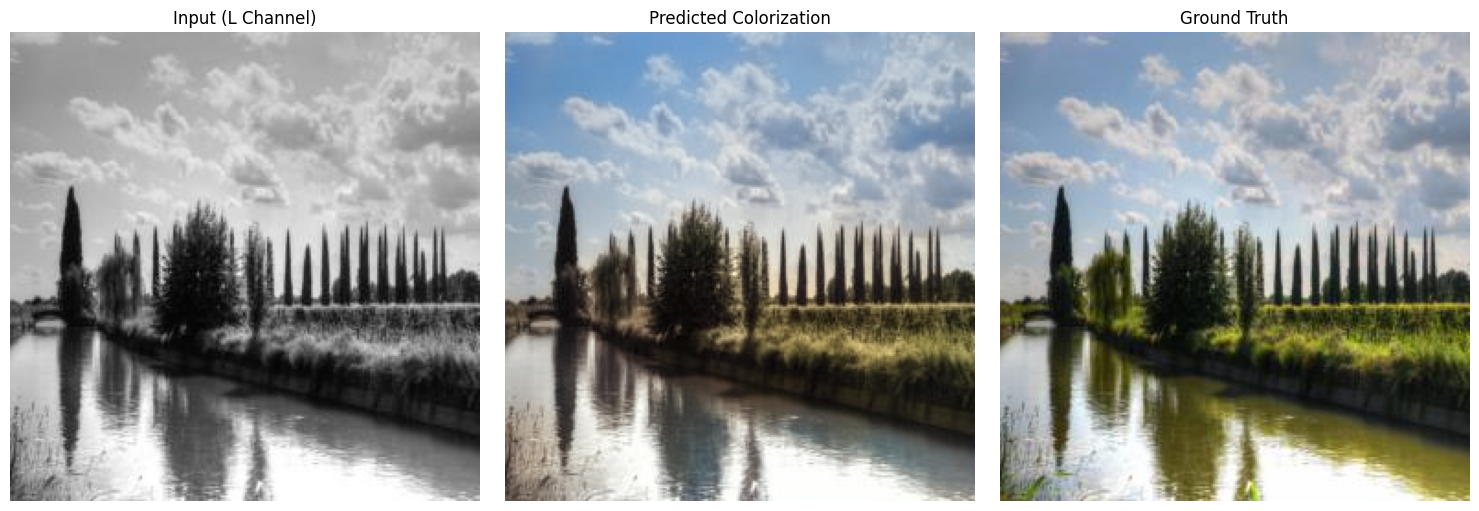
\includegraphics[width=0.9\linewidth]{Figs/landscape-result-example.png}
  \caption{Colourized output of a river bank scene with trees and sky. The model recovers vibrant blues and greens that closely match natural colour expectations.}
  \label{fig:landscape_comparison}
\end{figure}

Performance was less reliable on images of animals and humans, especially when the ground truth involved bright or saturated colours. This averaging effect was common in images 
with strong borders between different colours, as the loss function penalized deviations from average tones. In more extreme cases, such as in Figure~\ref{fig:final-model-turtle}, 
much of the turtle's shell and surrounding water are rendered grey, muting the scene overall.

\begin{figure}[htbp]
  \centering
  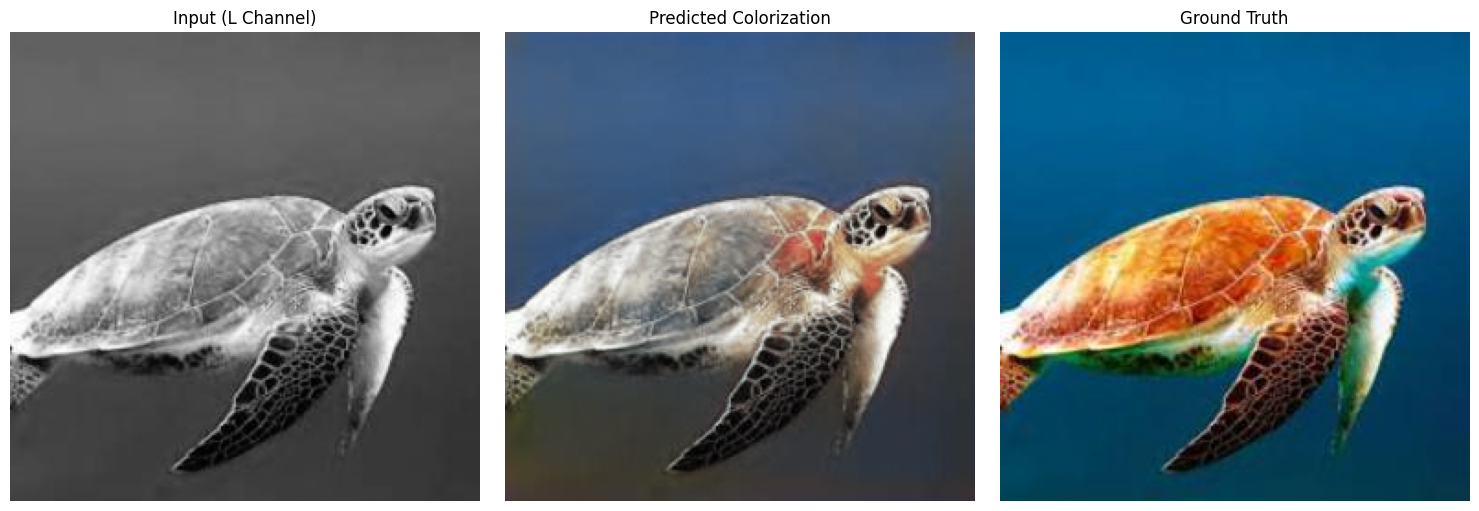
\includegraphics[width=0.9\linewidth]{Figs/turtle-result-example.png}
  \caption{Colourized output featuring a sea turtle. Large areas of the shell and surrounding water appear muted to grey, illustrating an averaging effect that reduces overall vibrancy.}
  \label{fig:final-model-turtle}
\end{figure}

We also experimented with alternate architectures including diverse colourization, quantized outputs using colour bins, multi-path networks, and exemplar-based models. Despite their 
conceptual appeal, these approaches often underperformed the original model. The exemplar and multi-path models frequently introduced a purple tint across diverse inputs, while the 
quantized and diverse variants still exhibited muted colours due to similar averaging tendencies. These results highlight that added architectural complexity does not guarantee improved 
performance and, in some cases, can introduce new  failure modes.

\begin{figure}[htbp]
  \centering
  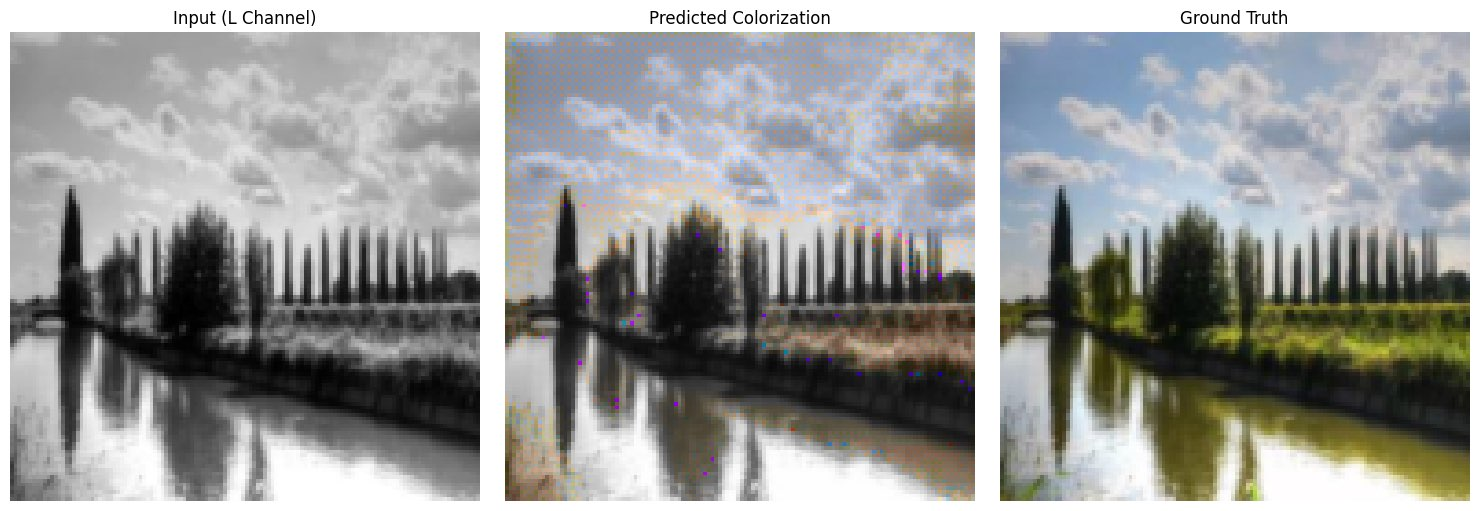
\includegraphics[width=0.9\linewidth]{Figs/colour-bins-landscape.jpg}
  \caption{Colour bin model output for a landscape scene. The image appears muted and lacks vibrancy, reflecting similar shortcomings observed in the original model's failure cases.}
  \label{fig:colour-bins-landscape}
\end{figure}

\section{Evaluation on New Data}
\label{new_data}

Our model was evaluated on a separate test set of 1,890 images, which were not used during training or validation. The model performed well relative to the validation results. Specifically, 
it achieved a final test loss of 0.007870, slightly higher than the validation loss of 0.007595. This indicates that the model generalizes well to unseen data, maintaining its ability to 
produce realistic colourizations across diverse image categories. Included below in Figure~\ref{fig:test-data-example} is an example of the model's performance on an image from the test 
dataset, demonstrating its ability to capture the scene's structure and colour distribution effectively.

\begin{figure}[htbp]
  \centering
  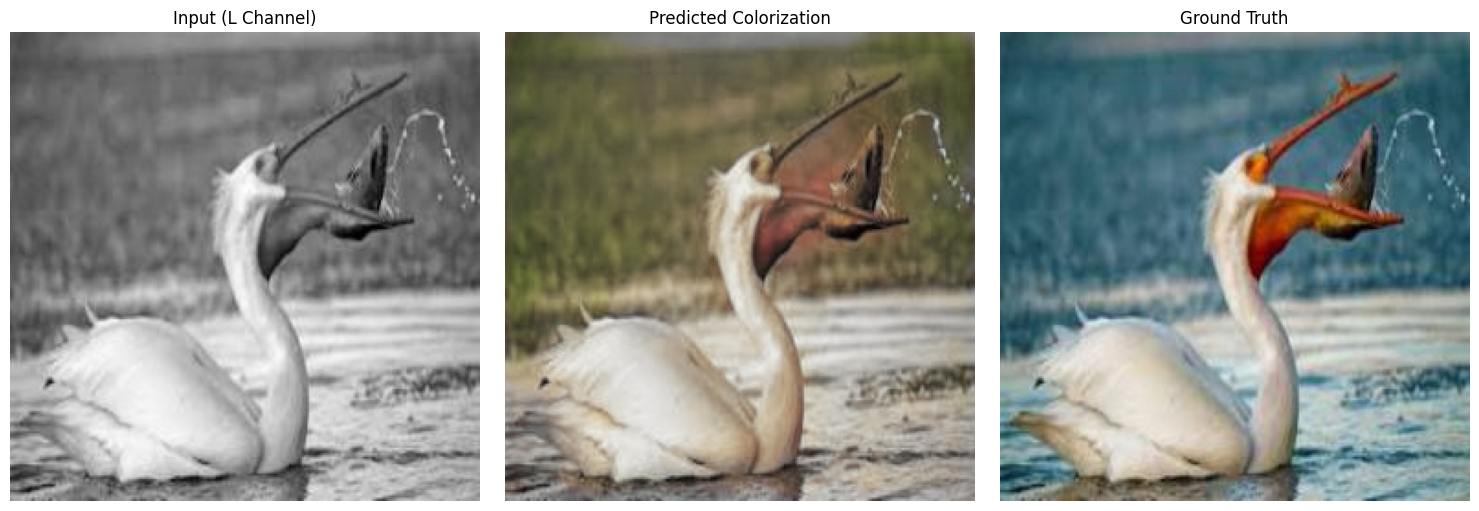
\includegraphics[width=0.95\linewidth]{Figs/test_data_result_example.png}
  \caption{Example result of the model on a test image, showing accurate structure and colour distribution.}
  \label{fig:test-data-example}
\end{figure}

\section{Discussion}
\label{discussion}

Our model generally performed well, particularly on landscape images, where predicted colours often aligned with the ground truth. This suggests the model successfully learned broad 
structural features such as skies, foliage, and terrain. Performance was weaker on images of humans and animals, especially when the ground truth contained multiple highly saturated 
colours. In these cases, both the baseline and primary model tended toward muted brownish tones. This behaviour likely stems from the pixel-wise loss, which encourages averaging to 
minimize error, producing desaturated outputs that reduce loss but compromise visual realism. Colour clustering on the dataset (Figure~\ref{fig:dom-colours}) shows that gray and brown 
tones dominate, which may have contributed to these muted outputs.

\begin{figure}[htbp]
  \centering
  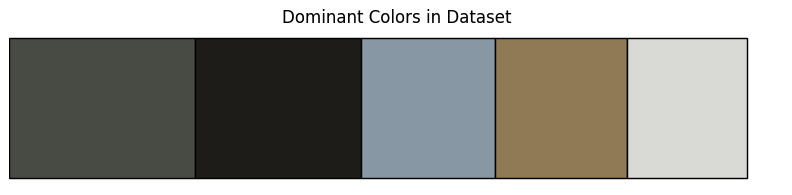
\includegraphics[width=0.95\linewidth]{Figs/dom-colours.png}
  \caption{The five dominant colours in the dataset identified using K-means clustering}
  \label{fig:dom-colours}
\end{figure}

We also explored alternative colourization approaches, including diverse colourization (generating multiple plausible outputs), quantized predictions using discrete colour bins, 
multi-path architectures, and exemplar-based methods. Despite their promise, these alternatives did not outperform the primary model in accuracy or visual quality. Multi-path and 
exemplar-based models often produced a noticeable purple hue, indicating instability or poor alignment between reference features and target content. Other methods continued to exhibit 
colour averaging, resulting in dull or brownish outputs.

These findings suggest that adding architectural complexity does not guarantee improvement. Some modifications introduced new artefacts, while others retained the same averaging tendencies. 
Overall, this highlights the importance of balanced architecture and careful tuning. Effective colourization depends not only on network design but also on the interaction between loss 
function, data distribution, and how these factors shape model outputs.

\pagebreak

\section{Ethical Considerations}
\label{ethical}

The dataset is publicly available, so there are no copyright or consent concerns. However, representation bias is possible if certain groups are overrepresented, such as lighter-skinned 
individuals, specific animal breeds, or particular fur colours. In such cases, the model may produce unrealistic or culturally insensitive colourizations. While these issues have not appeared 
in our outputs, they remain a potential risk, especially if colourized images are used for educational or identification purposes.

Evaluation bias is also a concern. Without knowledge of the dataset's demographic distribution, we cannot guarantee uniform model performance across all categories, which may skew metrics 
and misrepresent effectiveness.

Finally, because the model generates plausible but unverifiable outputs, users may place undue trust in the results. It is therefore important to communicate these limitations clearly and 
avoid applying the model in contexts that require factual accuracy.

\label{last_page}

\newpage
\bibliographystyle{iclr2022_conference}
\bibliography{APS360_Final_Report_ref}
\end{document}